\usetikzlibrary{shapes.geometric, arrows.meta, positioning, calc, shadows}
\tikzset{
  base/.style = {
    draw, thick, minimum height=1.2cm, minimum width=3.4cm,
    font=\sffamily, text centered, rounded corners=4pt
  },
  input/.style = {
    base, fill=blue!10, draw=blue!60, drop shadow
  },
  process/.style = {
    base, fill=green!10, draw=green!50!black, drop shadow
  },
  output/.style = {
    base, fill=red!10, draw=red!60, drop shadow
  },
  arrow/.style = {
    thick, -{Latex[length=3mm]}, line cap=round,
    shorten >=2pt
  }
}

\centering
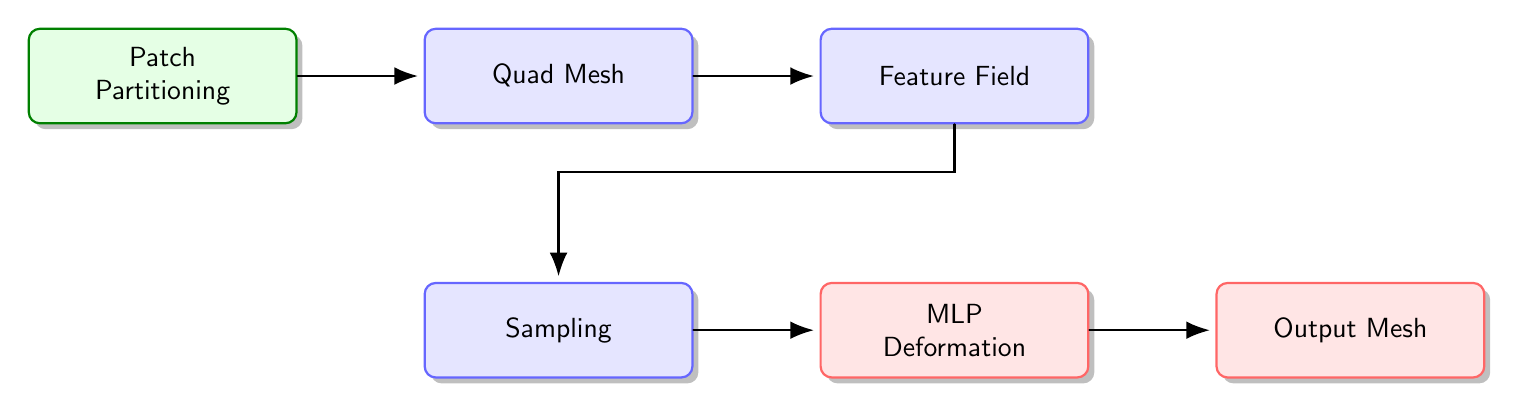
\begin{tikzpicture}[
  node distance = 2.2cm and 1.6cm,
  every node/.style = {align=center}
  ]

  % First row
  \node[process] (partition) {Patch\\Partitioning};
  \node[input, right=of partition] (quadmesh) {Quad Mesh};
  \node[input, right=of quadmesh] (featurefield) {Feature Field};

  % Second row
  \node[input, below=2cm of quadmesh] (sampling) {Sampling};
  \node[output, right=of sampling] (mlp) {MLP\\Deformation};
  \node[output, right=of mlp] (render) {Output Mesh};

  % Arrows top row
  \draw[arrow] (partition) -- (quadmesh);
  \draw[arrow] (quadmesh) -- (featurefield);

  % Arrows to second row
  \draw[arrow] (featurefield.south) -- ++(0,-0.6) -| (sampling.north);
  \draw[arrow] (sampling) -- (mlp);
  \draw[arrow] (mlp) -- (render);

\end{tikzpicture}

\vspace{-0.5em}
\captionof{figure}{Schematic of the processing pipeline. The input data undergoes patch partitioning and mesh structuring, followed by feature extraction. These are further processed through sampling and deformation stages to produce the final output mesh.}
\label{fig:teaser}
